\paragraph{QuizziPedia::Front-End::Directives::ExamModalityDirective}
\begin{figure} [ht]
	\centering
	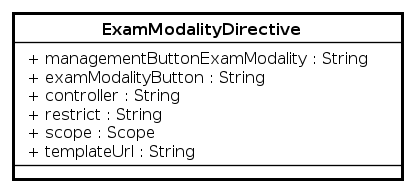
\includegraphics[scale=0.80]{UML/Classi/Front-End/QuizziPedia_Front-end_ExamModalityDirective.png}
	\caption{QuizziPedia::Front-End::Directives:ExamModalityDirective}
\end{figure} \FloatBarrier
\begin{itemize}
	\item \textbf{Descrizione}: \textit{directive} contenete i componenti grafici per attivare la modalità esame su un questionario e gestire le iscrizioni;
	\item \textbf{Utilizzo}: permette di attivare la modalità esame su un questionario e di gestirne le iscrizioni;
	\item \textbf{Relazioni con altre classi}:
	\begin{itemize}
		\item \textbf{IN \texttt{LangModel}}: rappresenta il modello delle informazioni per la giusta traduzione dell'applicazione;
		\item \textbf{IN \texttt{QuizEventModelView}}: classe di tipo \textit{modelview\ped{G}} la cui istanziazione è contenuta all'interno della variabile di ambiente \$scope di \textit{Angular\ped{G}}. All'interno di essa sono presenti le variabili e i metodi necessari per il \textit{Two-Way Data-Binding\ped{G}} tra le \textit{directives\ped{G}} \texttt{EliminationAndModifyDirective}, \texttt{ExamModalityDirective} e \texttt{QuestionnaireResul-\\tsDirective} e il \textit{controller\ped{G}} \texttt{QuizEventController};
		\item \textbf{OUT \texttt{QuestionnaireManagementView}}: \textit{view\ped{G}} principale per la gestione dei questionari.
	\end{itemize}
		\item \textbf{Attributi}:
		\begin{itemize}
			\item \texttt{+ managementButtonExamModality: String} \\ Attributo che viene utilizzato per visualizzare la giusta traduzione della \textit{label\ped{G}} per il bottone di gestione delle iscrizioni al questionario selezionato, in italiano o in inglese; 
			\item \texttt{+ examModalityButton: String} \\ Attributo che viene utilizzato per visualizzare la giusta traduzione della \textit{label\ped{G}} per il bottone di attivazione della modalità esame del questionario selezionato, in italiano o in inglese;
			\item \texttt{+ controller: String} \\ Stringa contenente il nome del \textit{controller\ped{G}} della direttiva;
			\item \texttt{+ restrict: String} \\ Stringa che permette di definire le modalità di inserimento della direttiva all'interno della pagina;
			\item \texttt{+ scope: Scope} \\ Oggetto scope interno della direttiva, contiene le funzionalità per gestire i dati presenti all'interno;
			\item \texttt{+ templateUrl: String} \\ Stringa contenente il percorso del file \textit{HTML\ped{G}} che contiene la direttive.
		\end{itemize}
\end{itemize}